%!TEX root = proyecto.tex

\lstset{frame=single,basicstyle=\ttfamily\small}

\chapter{Análisis de objetivos y metodología}

El COVID-19 es un virus que ha provocado en la humanidad incontables problemas, y en el mundo de la visión artificial también, por eso me voy a centrar en la creación de un prototipo que sea capaz de revisar el cumplimiento de las normas COVID impuestas en España y en todo el mundo por la OMS. Concretamente, detectar cuando una persona lleva, de manera correcta, una mascarilla al entrar a un comercio, cine, restaurante, etc. Los objetivos que se plantean para llevar esto a cabo son los siguientes:

\begin{itemize}
	\item Estudio de las tecnologías actuales, para comprobar su comportamiento con uso de mascarilla.
	\item Creación de un prototipo capaz de reconocer rostros y detectar si se lleva mascarilla.
	\item Estudiar la capacidad de que el prototipo pueda identificar si se lleva correctamente la mascarilla. 
	\item Poder detectar la mascarilla, independientemente del tipo que se lleve.
\end{itemize}

\section{Prototipo}

Para cada uno de los apartados del desarrollo de este \textit{TFG} se creará un prototipo con la finalidad de mostrar la tecnología expuesta en el mismo, con el objetivo final de crear una aplicación que contenga todos los prototipos y se puedan ejecutar de forma sencilla. 

Los prototipos serán probados en varios escenarios de prueba, todos ellos se realizarán en tiempo real. Se contará con una totalidad de tres escenarios:

\begin{itemize}
	\item Detección de mascarillas a una distancia cercana.
	\item Detección de mascarillas a una distancia media.
	\item Detección de mascarillas desde una posición alejada.
\end{itemize}

Asimismo, las pruebas se repetirán en dos dispositivos diferentes. El primero de ellos sin GPU y el segundo con GPU (CUDA). A continuación se muestran las especificaciones de los dispositivos:

\begin{table}[h!]
	\begin{center}
		\begin{tabular}{ |c|c|c|c| } 
			\hline
			 & PC 1 & PC 2 \\
			\hline
			\multirow{3}{4em}{CPU} & Intel i7-1065G7 & Intel i7-6700HQ \\ 
			& 1.30GHz & 2.60GHz \\ 
			& 8 núcleos & 8 núcleos \\ 
			\hline
			GPU & Intel Iris Plus Graphics  & GTX 980M 2Gb \\
			\hline
			CUDA & NO  & SI \\
			\hline
			RAM & 16 Gb & 8 Gb \\
			\hline
			OS & Ubuntu 18.04 & Ubuntu 18.04 \\
			\hline
		\end{tabular}
		\caption{Entornos de prueba.}
		\label{tab:table1}
	\end{center}
\end{table}

Por último, serán probados bajo un mismo \textit{dataset} (mostrado en el apartado \ref{dataset}) para calcular el porcentaje de aciertos que consiguen cada uno de ellos.

\section*{Herramientas}

Para el desarrollo del prototipo se hará uso del lenguaje de programación de alto nivel, Python. Junto a este se usarán las siguientes herramientas:

\begin{itemize}
	\item \textit{OpenCV}: Librería \textit{Open Source} centrada en la creación de aplicaciones en tiempo real sobre visión artificial, que cuenta con una gran cantidad de implementaciones de algoritmos de visión artificial.
	\item \textit{Dlib}: Librería compuesta por implementaciones de algoritmos \textit{Machine Learning}, centrada en la creación de aplicaciones que resuelven problemas del mundo real. En concreto se hará uso de su apartado de \textit{HOG detector} y \textit{Facial Landmark}.
	\item \textit{Scikit-learn}: Librería de \textit{Machine Learning} capaz de realizar clasificación, regresión, \textit{support vector machine} (SVM), \textit{gradient boosting, \textit{k-mean}}, etc. Se implementa conjuntamente con las librerías Numpy y SciPy.
	\item \textit{Numpy}: Librería que añade funcionalidad a \textit{arrays} multidimensionales y matrices, junto a un gran conjunto de operaciones matemáticas para trabajar con ellos.
	\item \textit{Mediapipe}: Librería con soluciones y aplicaciones de \textit{Machine Learning} para dispositivos móviles, en la nube o web.
	\item \textit{Tensorflow}: Librería de \textit{Machine Learning}, referente a el entrenamiento y utilización de redes convolucionales (\textit{Deep Learning}).
\end{itemize}

\vspace{-0.5cm}
\section*{Fases de desarrollo}

El proceso de implementación del prototipo en cada una de las técnicas presentadas en este TFG, van a contar con el siguiente flujo de trabajo:

\begin{enumerate}
	\item \textit{Investigación}: El primer paso, se centra en la investigación del funcionamiento de la técnica a estudiar. Priorizando el estudio del \textit{paper}, artículo oficial donde se presenta la técnica por sus autores. Y, posteriormente buscar información extra en libros u artículos web.
	\item \textit{Implementación básica}: EL segundo paso se trata de realizar una implementación de la técnica estudiada, tal y como se presenta por los autores. Con el objetivo de realizar un estudio de precisión y rapidez.
	\item \textit{Implementación propia}: Por último, se crea un prototipo de la técnica intentando resolver los objetivos establecidos. Recabando datos, para una comparación final entre todas las técnicas estudiadas.
\end{enumerate}

\section*{Dataset} \label{dataset}

Un \textit{dataset} es un conjunto de imágenes utilizado para realizar el entrenamiento y validación de un modelo de \textit{Machine Learning}. En este trabajo se hará uso de la combinación de dos \textit{dataset} existentes para representar todas las posibilidades del problema planteado, conteniendo imágenes de personas con mascarilla, sin ella y con ella pero mal colocada. El primer dataset de la combinación proviene de \textit{Kaggle} llamado \textit{Covid face mask detection dataset} \cite{datasetMask} (Figura \ref{fig:1}). Kaggle es una comunidad de \textit{Machine Learning} y \textit{Deep Learning} donde se comparten proyectos y dataset. Mientras que, el segundo dataset proviene de una investigación \cite{Cabani_2021}, llamada \textit{Maskedface-net}, centrada en la creación de imágenes de personas donde se muestre un mal uso de la mascarilla (Figura \ref{fig:1c}). Finalmente, el dataset creado para este trabajo cuenta con un total de 895 imágenes, donde 745 formarán el conjunto de entrenamiento y 150 el de test.

\begin{figure}[htp]
	\centering
	\begin{subfigure}{0.2\linewidth}
		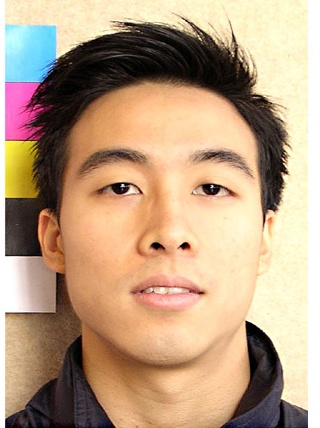
\includegraphics[width=\linewidth]{imagenes/dataset1-1.jpg} 
		\caption{}
		\label{fig:1a}
	\end{subfigure}\hfill
	\begin{subfigure}{0.2\linewidth}
		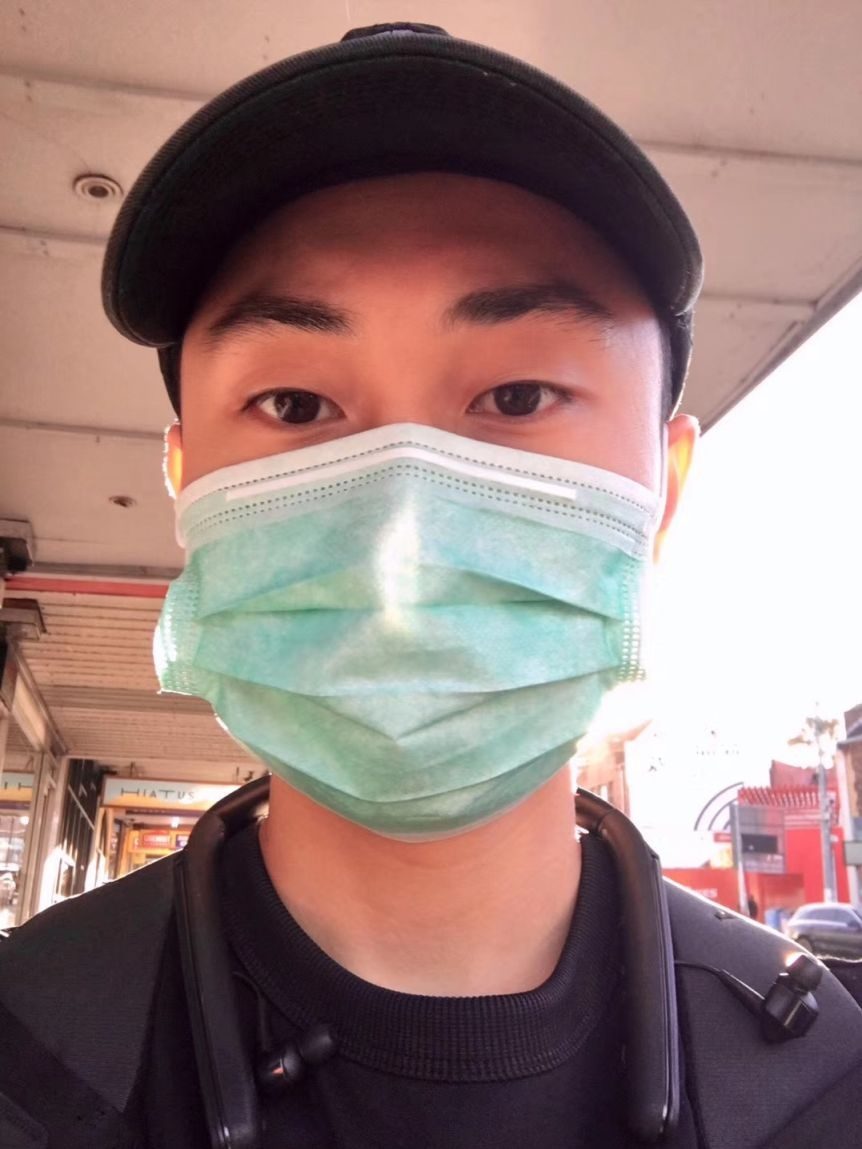
\includegraphics[width=\linewidth]{imagenes/dataset1-2.jpg}
		\caption{}
		\label{fig:1b}
	\end{subfigure}\hfill	
	\begin{subfigure}{0.2\linewidth}
		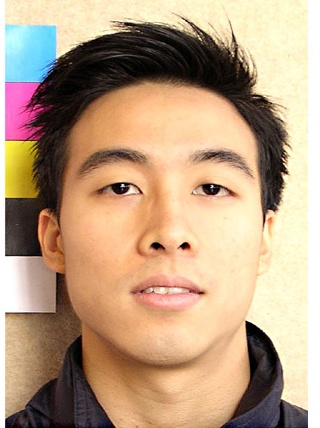
\includegraphics[width=\linewidth]{imagenes/dataset1-1.jpg}
		\caption{}
		\label{fig:1c}
	\end{subfigure}
	\caption{Ejemplos de imágenes del dataset 1 (\ref{fig:1a}, \ref{fig:1b}) y del dataset 2 (\ref{fig:1c}).}
	\label{fig:1}
\end{figure}


